The three dimensional geometry of the non-premixed swirl combustor chamber an it's central cross-sectional dimensions are presented in \autoref{fig:model_rql}. The combustion chamber constitutes 
of a rich burn region with a fuel inlet at the centre. The ring around the fuel inlet is the primary air inlet. There are 16 air holes downstream of the combustion chamber 
to deliver the secondary air for the lean combustion zone. The combustion chamber has been designed in such a way that for specific mass flows, rich combustion can take place
in the rich region and after adding the secondary air, the NOx can be reduced using lean combustion.

\subsection{Boundary Conditions}

The equivalence ratio of the primary combustion zone has been set to 1.24 and the global equivalence ratio has been set to 0.42. Both of these quantities are design choices
and have helped derive the combustor geometry. The fuel and air temperature used for this study have been adopted from reference \cite{wang2023non}. The combustor specifications
and the boundary conditions are summarized in \autoref{tab:air_fuel_properties}. The fuel pressure has been set higher that the air pressure to avoid back flow.

\begin{table}[H]
    \centering
    \caption{Boundary conditions.}\label{tab:air_fuel_properties}
    \begin{tabular}{lcc}
    \toprule
    & Temperature [K] & Pressure [MPa] \\
    \midrule
    Air  & 800  & 12 \\
    Fuel & 325  & 15 \\
    \bottomrule
    \end{tabular}
\end{table}

The following subsections discuss the conditions at the two different zones of combustion in detail. An important parameter to note here is the momentum flux ratio ($J$).
The momentum flux ratio is a critical parameter in combustion systems, defined as the ratio of momentum flux of the fuel to that of the air. It influences flame stability, mixing, and combustion efficiency. Mathematically, it can be defined as:

\begin{equation}
    J = \frac{\rho_{\text{jet}} u_{\text{jet}}^2}{\rho_{\infty} u_{\infty}^2}
\end{equation}

\subsection{Rich Burn Zone}

As mentioned before, the equivalence ratio for the rich burn zone has been set to $\phi_{\text{rich}} = 1.24$ as a design choice.
Literature \cite{Talpallikar1992} suggests that an acceptable $J$ for a inlet swirl type combustor should be between 2-3, which has been set as a constraint for this design.


Writing the balanced chemical equation:


\begin{equation}
    \ce{4NH3 + 3(O2 + 3.76 N2) -> 2N2 + 6H2O + 11.28N2}\label{eq:balanced_reaction}
\end{equation}

In \autoref{eq:balanced_reaction}, the oxidizer nitrogen is kept separate from the inert air nitrogen to keep track. The air-fuel ratio can be expressed as:

\begin{equation}
    \left( \frac{A}{F} \right) = \frac{N_{\text{air}}}{N_{\text{fuel}}} \times \frac{MW_{\text{air}}}{MW_{\text{fuel}}}
\end{equation}

From the balanced reaction in \autoref{eq:balanced_reaction}:

\begin{equation}
    \left( \frac{A}{F} \right)_{\text{stoic}} = 4.76 \times 0.75 \times \frac{28.85 \; \text{g/mol}}{17.034 \; \text{g/mol}} = 6.05
\end{equation}


Therefore, using the above relation, the air-fuel ratio for a rich combustion configuration can be obtained:

\begin{equation}
    \phi = \frac{(A/F)_{\text{stoic}}}{(A/F)_{\text{required}}}
\end{equation}

The required air-fuel ratio for $\phi = 1.24$ is computed as follows:

\begin{equation}
    (A/F)_{\text{required}} = \frac{(A/F)_{\text{stoic}}}{\phi} = \frac{6.05}{1.25} = 4.854
\end{equation}

Therefore, $\phi$ and $(A/F)$ have been set for the rich combustion have been set so far. The next step is to obtain the inlet mass flow rates for the 
fuel and the air for this design. It is known that $\dot{m} = \rho V A$. Area is known from the geometry. $\rho$ for air and fuel can be obtained from the respective fluid properties. Hence,
the mass flow for both the air and fuel can be obtained using the respective inlet velocities. A range for both $U_{\text{air}}$ and $U_{\text{fuel}}$ as well as $J$ have been used:

\begin{table}[H]
\centering
    \begin{tabular}{ll}
         $J$              &  2 - 3 \\
         $U_{\text{air}}$ &  40 m/s to 90 m/s \\
        $U_{\text{fuel}}$ &  60 m/s to 110 m/s \\
    \end{tabular}
\end{table}

After iterating over the above ranges, the results are filtered based on the required $\phi$ and $J$. The program used has been presented in Appendix \ref{subsection:primary_calcs}.
The chosen operating conditions for this region are presented in \autoref{tab:air_fuel_properties}. The program helps obtain the inlet mass flow rates for the fuel and the oxidizer. The results used in the analysis presented in this report are below:

\begin{table}[H]
    \centering
    \begin{tabular}{ll}
         Primary inlet mass flow rate &  0.035631 kg/s\\
         Fuel mass flow rate &  0.007339 kg/s
    \end{tabular}
\end{table}


These conditions have been used to set the boundary conditions for the numerical analysis which will be discussed in a later section.


\subsection{Lean Burn Zone}

Literature suggests that a momentum flux ratio of 40 in the mixing zone should induce enough turbulence in the zone to mix the secondary air with the downstream gases from the rich combustion zone. Therefore, the momentum flux ratio for this region has be set to 40 as a design choice \cite{Talpallikar1992, Lefebvre2010}. The objective is to calculate the secondary mass flow rate such the the global equivalence ratio becomes 0.42. This can be obtained by computing the global air-fuel ratio:

\begin{equation}
\begin{split}
        \left( A/F \right)_{\text{global}} & = \left( A/F \right)_{\text{stoic}} / \phi_{\text{global}} \\
        & = 4.854 / 0.42 \\
        & = 14.3993
\end{split}
\end{equation}

Then, the global mass flow rate can be calculated as:



\begin{equation}
\begin{split}
        \dot{m}_{\text{global}} & = \dot{m}_{F} \times  \left( A/F \right)_{\text{global}} \\
        & = 0.007339 \times 14.3993 \\
        & = 0.07004 \text{ kg/s}
\end{split}
\end{equation}

Therefore, a secondary mass flow rate of 0.07004 kg/s leads to a global equivalence ratio of 0.42 after the mixing/quench region.

\subsection{Swirler Design}

The primary zone airflow pattern is of prime importance to flame stability. For better mixing, one of the most effective ways of inducing flow recirculation in the primary zone is to fit a swirler in the dome around the fuel injector. This causes recirculation in the core region when the amount of rotation imparted to the flow is high. There are two main types of air swirles: axial and radial. In the presented design, an axial swirler is used. This is because it rotates the flow better in the tangential direction allowing it to evenly mix with the fuel jets. Typical ranges of values for the design of axial swirlers are \cite{dodds1990combustion, knight1953component}

\begin{table}[H]
    \centering
    \begin{tabular}{lll}
        \textbf{Parameter} & \textbf{Typical Value} & \textbf{Selected} \\
         Vane angle, $\theta$ &  30 - 60 deg & 45 deg \\
         Vane thickness, $t_{\nu}$ & 0.7 - 1.5 mm & 1.5 mm \\
         Number of Vanes, $n_{\nu}$ & 8 - 16 & 8
    \end{tabular}
\end{table}

\subsection{Final Design}

The general design of an RQL combustor has been adopted from existing designs being tested with ammonia as the fuel. One such design is presented in reference \cite{FATEHI20241} and shown in \autoref{fig:ref_rql_combustor}. It must be noted that the combustor used in this analysis is based on the reference combustor, however, many aspected have been changed. For example, the sleeve for the secondary air is replaced with a simple secondary air inlet zone and the while secondary air region has been removed for simplicity. 

\begin{figure}[H]
    \centering
    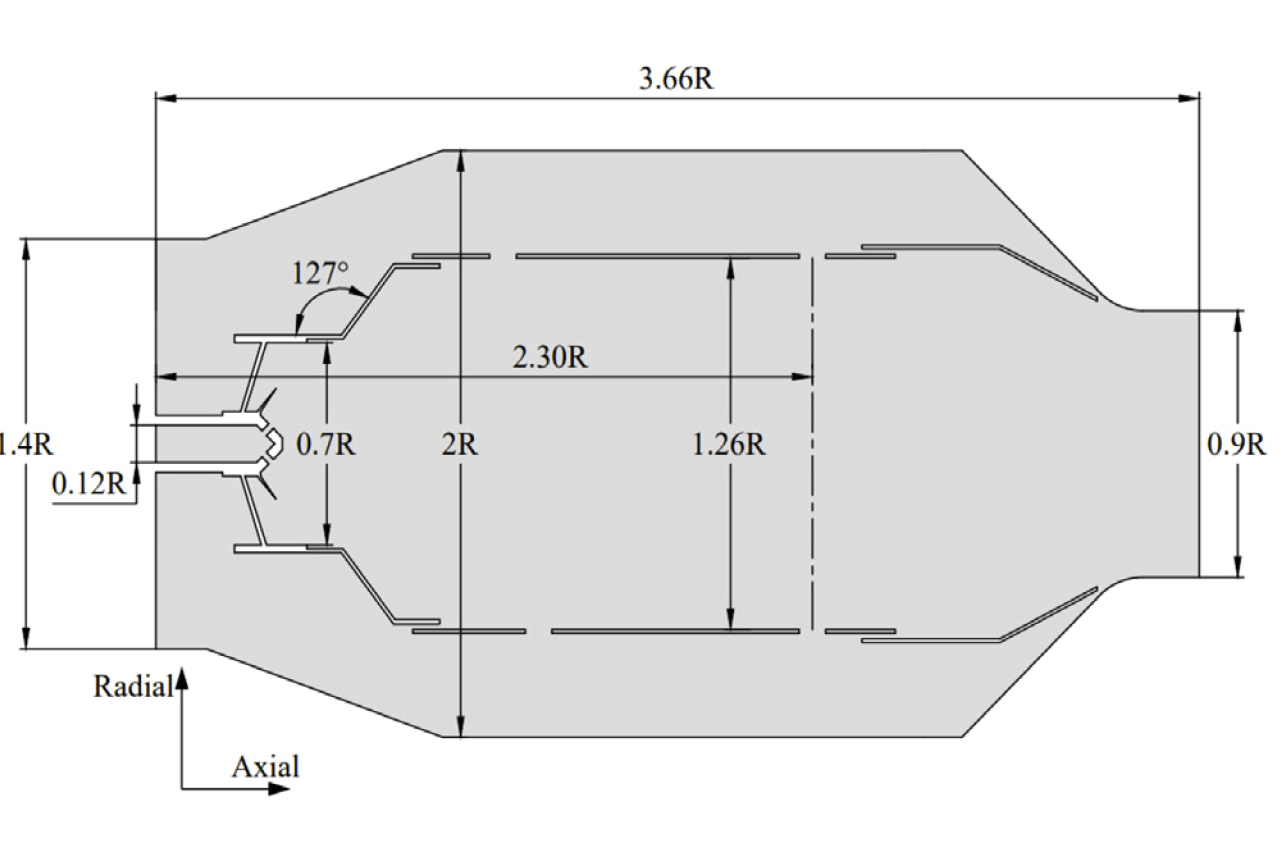
\includegraphics[width=0.5\linewidth]{figs/reference_rql_combustor.png}
    \caption{Central cross-sectional dimensions of the reference non-premixed swirl combustor \cite{samuelsen2006rich}.}\label{fig:ref_rql_combustor}
\end{figure}

Based on the analysis discussed in the previous sections, an RQL combustor is modelled and shown in \autoref{fig:model_rql}. The left figure shows the overall design and the right figure shows the details of the fuel injector. A detailed drawing with all the dimensions is presented in Appendix \ref{subsection:rql_dim_drawing}.

\begin{figure}[H]
    \centering
    \begin{subfigure}{0.49\linewidth}
      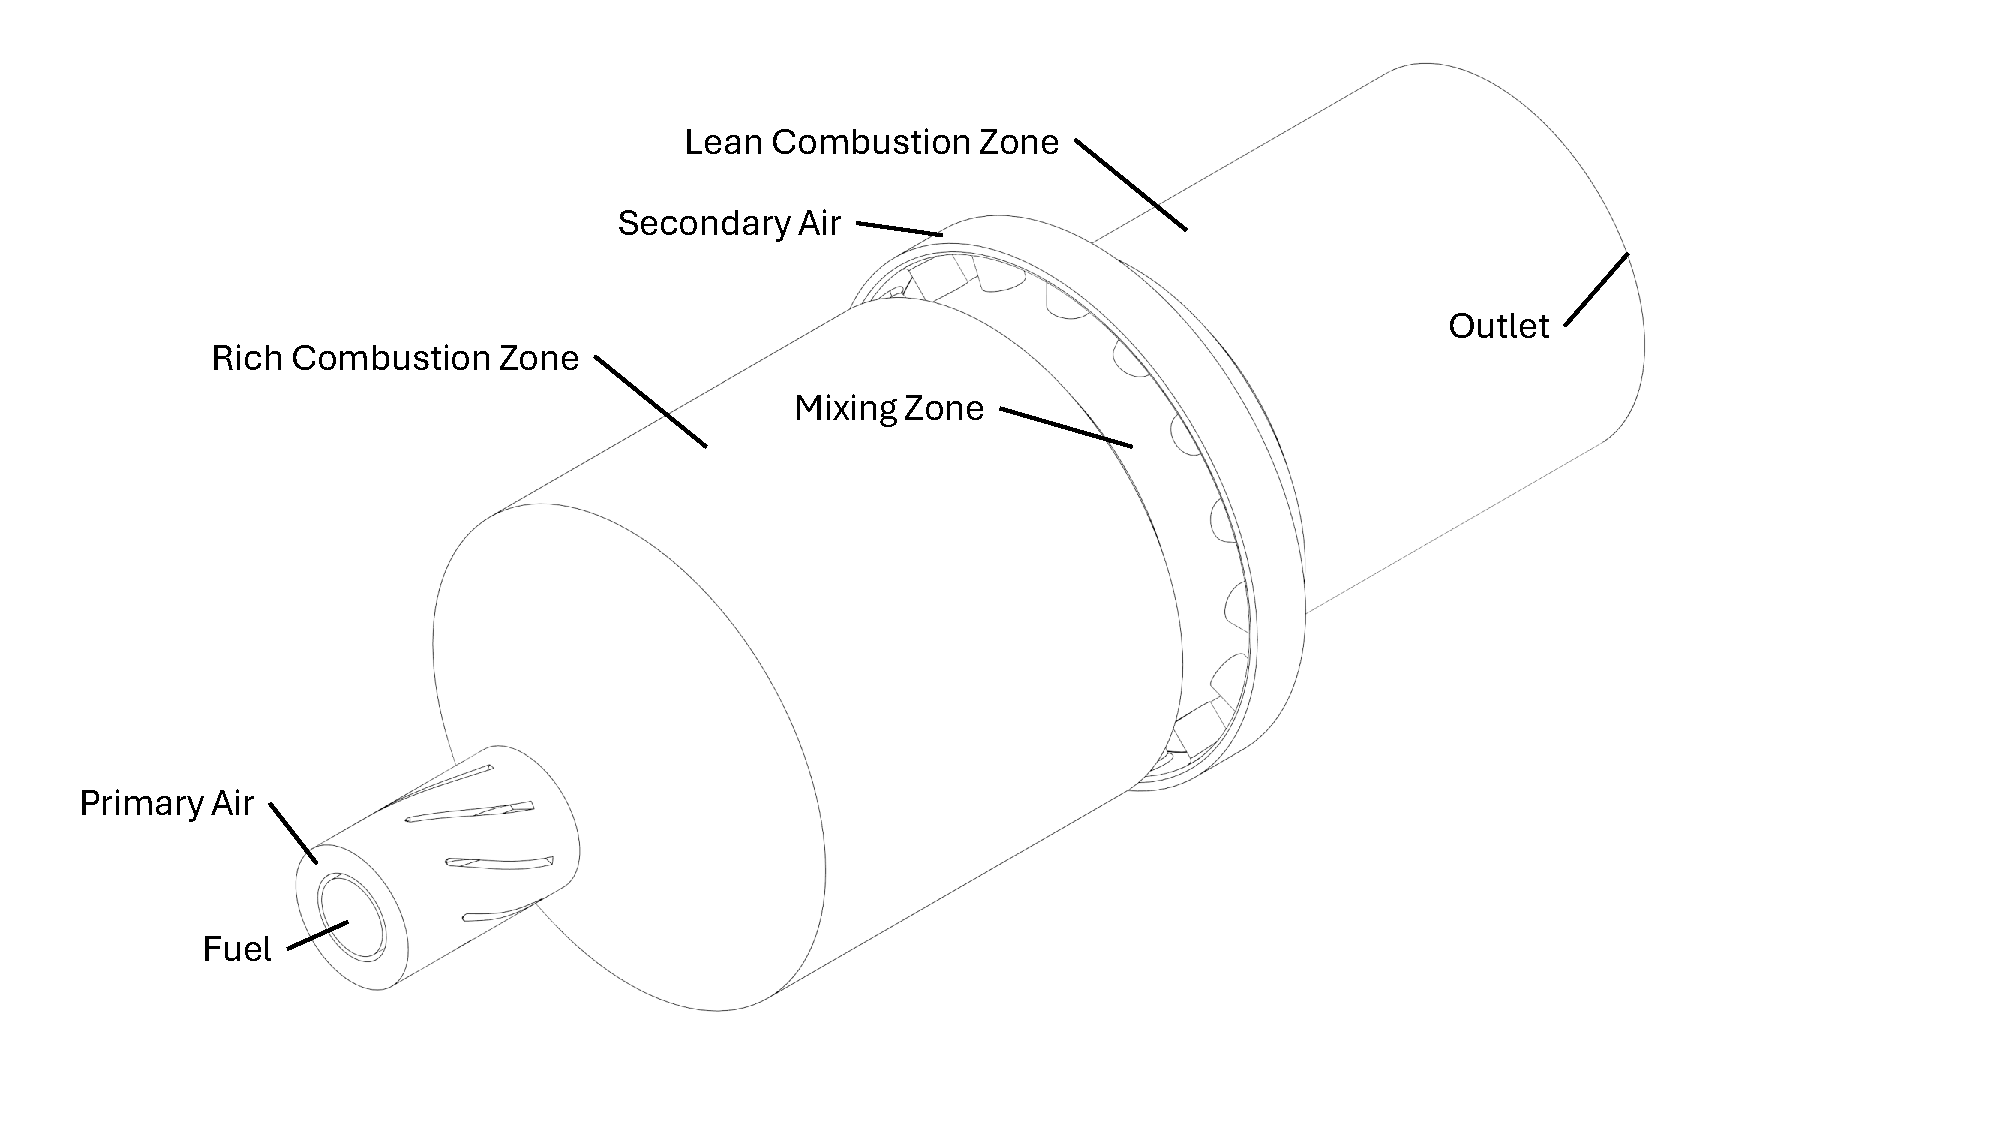
\includegraphics[width=\linewidth]{figs/overall_design.pdf}
    \end{subfigure}
    \hfill
    \begin{subfigure}{0.49\linewidth}
      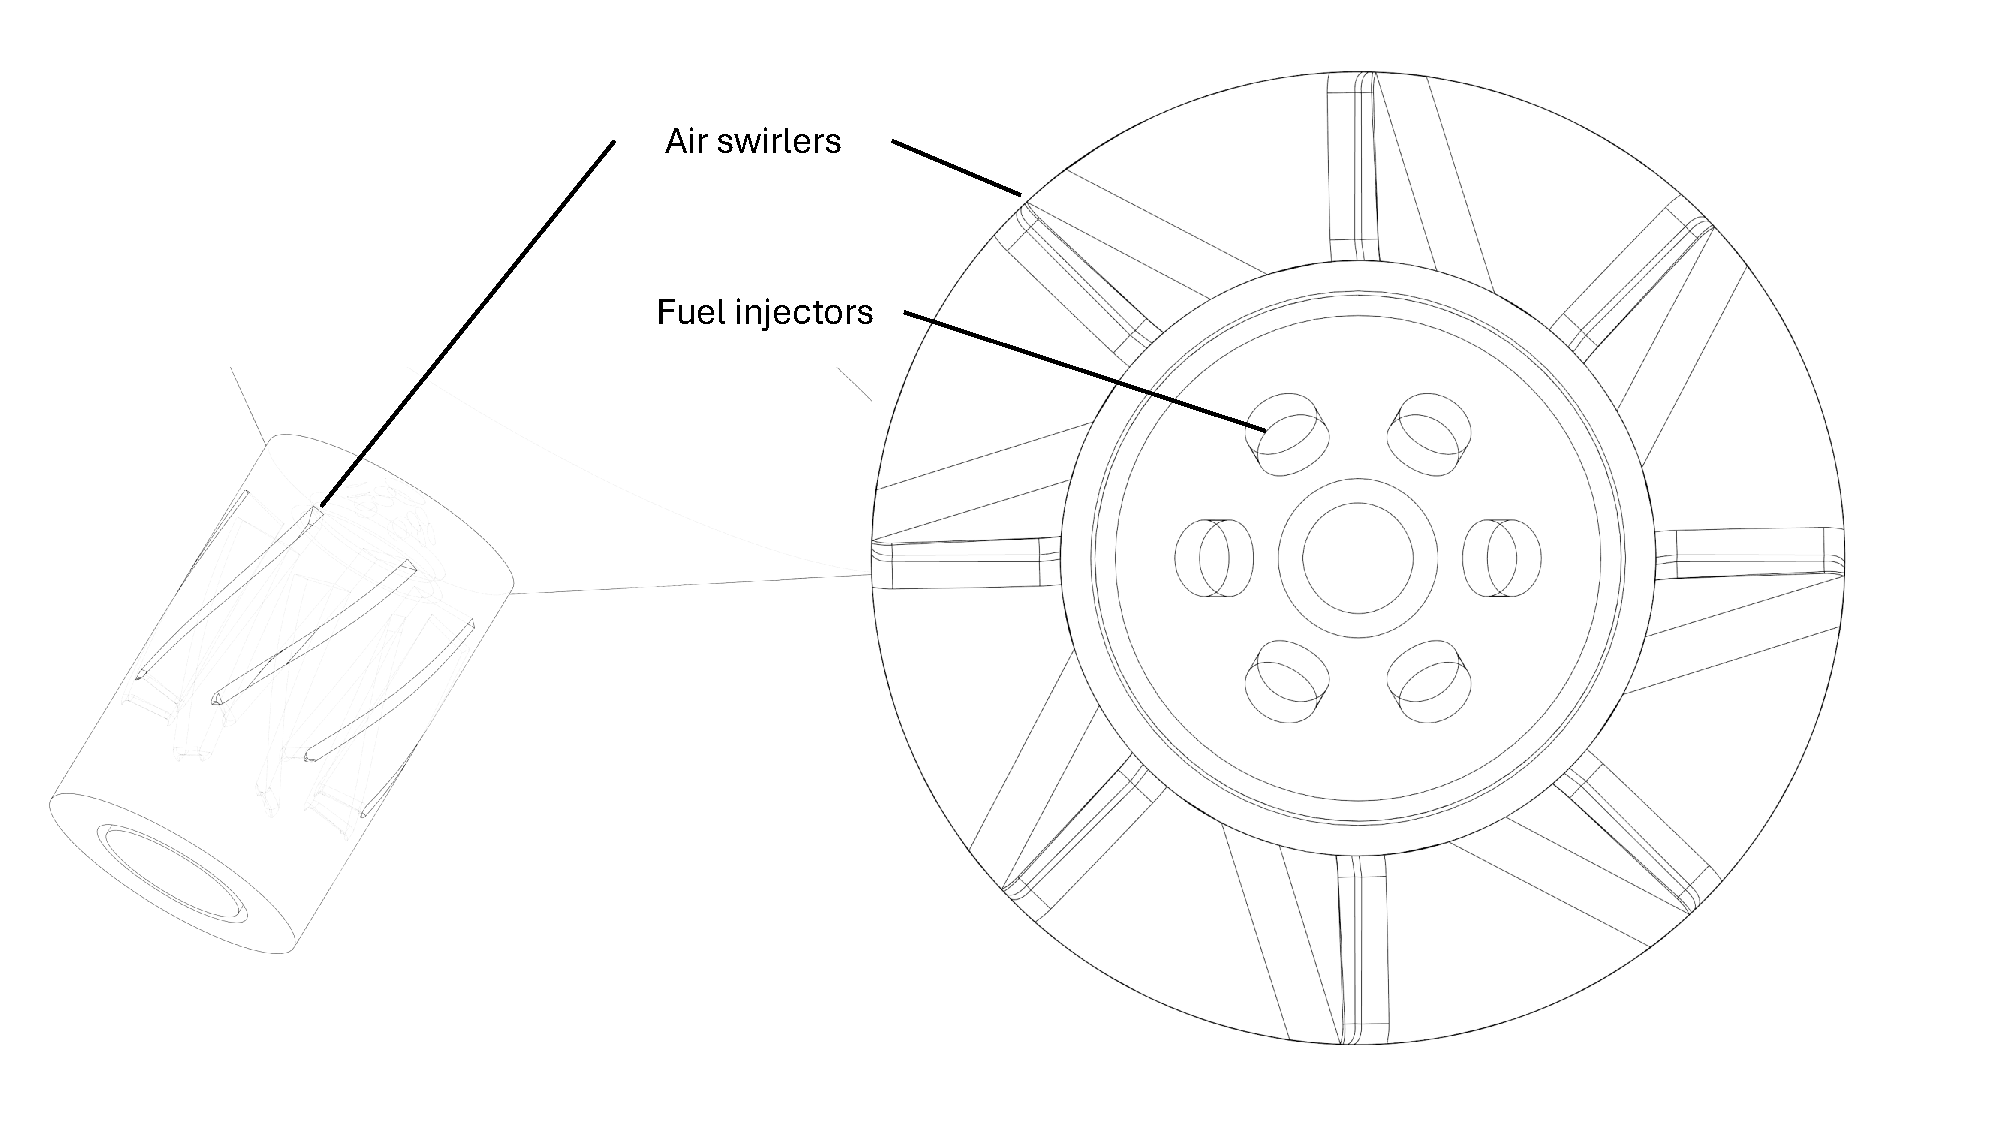
\includegraphics[width=\linewidth]{figs/injector.pdf}
    \end{subfigure}
\caption{Three dimensional model of the designed combustor.}\label{fig:model_rql}
\end{figure}



